\documentclass[12pt, a4paper]{book}

\usepackage[T1]{fontenc}
\usepackage[utf8]{inputenc}
\usepackage[charter, cal=cmcal]{mathdesign}
\usepackage[scaled=0.92]{helvet}
\usepackage{geometry}
\geometry{a4paper, top=30mm, bottom=30mm, inner=32mm, outer=25mm, marginparwidth=18mm}

\usepackage{amsmath, amsthm}
\usepackage[version=4]{mhchem}
\usepackage{graphicx}
\usepackage{xcolor}
\usepackage{tikz}
\usetikzlibrary{arrows.meta, shapes.geometric, positioning, calc, backgrounds}
\usepackage{pgfplots}
\pgfplotsset{compat=1.18}
\usepackage{tcolorbox}
\tcbuselibrary{skins, breakable, theorems}
\usepackage{titlesec}
\usepackage{fancyhdr}
\usepackage{enumitem}
\usepackage{booktabs}
\usepackage{array}
\usepackage{parskip}
\usepackage{siunitx}
\usepackage[colorlinks=true, linkcolor=BrickRed,
            urlcolor=NavyBlue, citecolor=ForestGreen]{hyperref}

% ── Colours (Journey 6 — forest green / amber) ────────────────────────────────
\definecolor{JourneyColor}{HTML}{065F46}
\definecolor{ModuleColor}{HTML}{059669}
\definecolor{PuzzleColor}{HTML}{B45309}
\definecolor{DiscoveryColor}{HTML}{D97706}
\definecolor{WarningColor}{HTML}{991B1B}
\definecolor{ProblemColor}{HTML}{6B21A8}
\definecolor{ReflectColor}{HTML}{0D9488}
\definecolor{HistoryColor}{HTML}{78350F}

% ── Boxes ─────────────────────────────────────────────────────────────────────
\newtcolorbox{puzzlebox}[1][]{enhanced,breakable,
  colback=PuzzleColor!6,colframe=PuzzleColor,fonttitle=\bfseries\sffamily,
  title={The Puzzle},attach boxed title to top left={yshift=-2mm,xshift=6mm},
  boxed title style={colback=PuzzleColor},borderline west={3pt}{0pt}{PuzzleColor},#1}

\newtcolorbox{discoverybox}[1][]{enhanced,breakable,
  colback=DiscoveryColor!8,colframe=DiscoveryColor,fonttitle=\bfseries\sffamily,
  title={Discovery},attach boxed title to top left={yshift=-2mm,xshift=6mm},
  boxed title style={colback=DiscoveryColor},borderline west={3pt}{0pt}{DiscoveryColor},#1}

\newtcolorbox{problembox}[1][]{enhanced,breakable,
  colback=ProblemColor!5,colframe=ProblemColor,fonttitle=\bfseries\sffamily,
  title={Problems},attach boxed title to top left={yshift=-2mm,xshift=6mm},
  boxed title style={colback=ProblemColor},borderline west={3pt}{0pt}{ProblemColor},#1}

\newtcolorbox{deepbox}[1][]{enhanced,breakable,
  colback=JourneyColor!5,colframe=JourneyColor,fonttitle=\bfseries\sffamily,
  title={Deep Problems},attach boxed title to top left={yshift=-2mm,xshift=6mm},
  boxed title style={colback=JourneyColor},borderline west={4pt}{0pt}{JourneyColor},#1}

\newtcolorbox{historybox}[1][]{enhanced,breakable,
  colback=HistoryColor!7,colframe=HistoryColor!60,fonttitle=\bfseries\sffamily\small,
  title={Historical Note},attach boxed title to top left={yshift=-2mm,xshift=6mm},
  boxed title style={colback=HistoryColor!80},#1}

\newtcolorbox{reflectionbox}[1][]{enhanced,breakable,
  colback=ReflectColor!6,colframe=ReflectColor,fonttitle=\bfseries\sffamily,
  title={Reflection},attach boxed title to top left={yshift=-2mm,xshift=6mm},
  boxed title style={colback=ReflectColor},borderline west={3pt}{0pt}{ReflectColor},#1}

\newtcolorbox{namedconcept}[2][]{enhanced,
  colback=ModuleColor!6,colframe=ModuleColor,fonttitle=\bfseries\sffamily\large,
  title={#2},attach boxed title to top left={yshift=-2mm,xshift=6mm},
  boxed title style={colback=ModuleColor},#1}

% ── Section formatting ────────────────────────────────────────────────────────
\titleformat{\chapter}[display]
  {\normalfont\sffamily\huge\bfseries\color{JourneyColor}}
  {\textcolor{JourneyColor!60}{\chaptertitlename\ \thechapter}}{10pt}{\Huge}
  [\vspace{2pt}\textcolor{JourneyColor}{\titlerule[1.5pt]}]
\titleformat{\section}
  {\normalfont\sffamily\Large\bfseries\color{ModuleColor}}
  {\thesection}{1em}{}[\textcolor{ModuleColor!40}{\titlerule[0.6pt]}]
\titleformat{\subsection}
  {\normalfont\sffamily\large\bfseries\color{JourneyColor!80}}{\thesubsection}{1em}{}
\titleformat{\subsubsection}
  {\normalfont\sffamily\normalsize\bfseries}{\thesubsubsection}{1em}{}

\pagestyle{fancy}
\fancyhf{}
\fancyhead[LE]{\small\sffamily\textcolor{JourneyColor}{\leftmark}}
\fancyhead[RO]{\small\sffamily\textcolor{ModuleColor}{\rightmark}}
\fancyfoot[C]{\small\thepage}
\renewcommand{\headrulewidth}{0.4pt}

\newcommand{\newterm}[1]{\textit{\textcolor{DiscoveryColor}{#1}}}
\newcommand{\important}[1]{\textcolor{ModuleColor}{\textbf{#1}}}

\begin{document}

\setcounter{chapter}{5}
\chapter[Journey 6 --- Organic Chemistry: Carbon's Grammar]
        {Journey Six\\[8pt]
         \textcolor{ModuleColor}{\large Organic Chemistry: Carbon's Grammar}}
\setcounter{section}{3}

\section{Module 6.4 --- Electron Flow and Reaction Mechanisms}
\label{sec:mod6.4}

\subsection*{Motivation}

We explored in Module 6.1 and 6.2 how carbon hybridizes to form 3D geometries, and in Module 6.3 how delocalized electrons stabilize aromatic structures.
Now, we study chemical change: how organic molecules react to form new configurations.

Organic reaction mechanisms are not memorized lists of facts.
They are governed by a precise, universal grammar: the flow of electrons from regions of high electron density to regions of low electron density.
This flow is represented by **curved arrows**.
This module explores this grammar through nucleophilic substitution and elimination reactions.
We will discover how minor changes in reactant structures completely rewrite the kinetics, transition states, and stereochemical shapes of products.

\subsection{The Kinetic substitution Divergence}

We investigate a kinetic mystery in basic organic substitution reactions.

\begin{puzzlebox}
\textbf{The Substitution rate Laws.}

Consider two substitution reactions where a bromide leaving group ($\ce{Br-}$) is replaced by a hydroxide nucleophile ($\ce{OH-}$):
* **Reaction 1:** Methyl bromide with hydroxide:
  \[
    \ce{CH3Br + OH- -> CH3OH + Br-}.
  \]
  The measured rate law is bimolecular: $R = k_1 [\ce{CH3Br}][\ce{OH-}]$.
* **Reaction 2:** *tert*-butyl bromide with hydroxide:
  \[
    \ce{(CH3)3CBr + OH- -> (CH3)3COH + Br-}.
  \]
  The measured rate law is unimolecular: $R = k_2 [\ce{(CH3)3CBr}]$.
  Increasing the concentration of hydroxide has completely no effect on the speed of Reaction 2!
\begin{enumerate}[label=(\alph*), leftmargin=*]
  \item Why does the rate of Reaction 1 depend on the concentration of both reactants, whereas Reaction 2 is independent of the nucleophile concentration?
  \item In organic chemistry, we use **curved arrows** to trace the movement of electron pairs. An arrow starts at an electron source (a lone pair or bond) and points to an electron sink.
        Identify the **nucleophile** (electron-rich species) and the **electrophile** (electron-poor species) in both reactions.
  \item We define two pathways:
        * **$S_N2$ (Substitution Nucleophilic Bimolecular):** A single-step concerted backside attack.
        * **$S_N1$ (Substitution Nucleophilic Unimolecular):** A multi-step mechanism where the leaving group departs first to form a carbocation intermediate.
        Which mechanism corresponds to Reaction 1? Which to Reaction 2?
\end{enumerate}
\end{puzzlebox}

\subsection{The $S_N2$ Mechanism: Concerted Inversion}

We study the dynamics and stereochemistry of the concerted substitution pathway.

\begin{explobox}
In an $S_N2$ reaction, the nucleophile attacks the carbon from the exact opposite side of the leaving group (backside attack).
\begin{center}
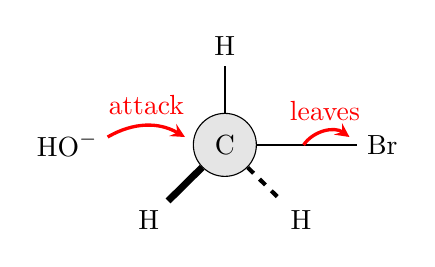
\begin{tikzpicture}[scale=1.0]
  % SN2 mechanism curved arrow
  \node (Nu) at (-2.0, 0) {$\ce{HO^-}$};
  \node[circle, draw, fill=gray!20, minimum size=0.8cm] (C) at (0,0) {C};
  \node (Br) at (2.0, 0) {$\ce{Br}$};
  \node[above=0.6cm of C] (H1) {H};
  \node[below left=0.6cm of C] (H2) {H};
  \node[below right=0.6cm of C] (H3) {H};
  
  \draw[thick] (C) -- (Br);
  \draw[thick] (C) -- (H1);
  \draw[line width=2.5pt] (C) -- (H2);
  \draw[dashed, line width=1.5pt] (C) -- (H3);
  
  % Curved arrow from HO lone pair to C
  \draw[->, >=stealth, line width=1.2pt, red, bend left=30] 
    ($(Nu.east) + (0, 0.1)$) to node[above] {attack} ($(C.west) + (-0.1, 0.1)$);
  % Curved arrow from C-Br bond to Br
  \draw[->, >=stealth, line width=1.2pt, red, bend left=45] 
    (1.0, 0) to node[above] {leaves} ($(Br.west) + (-0.1, 0.1)$);
\end{tikzpicture}
\end{center}
\begin{enumerate}[label=(\alph*), leftmargin=*]
  \item Explain why the backside attack is stereospecific, forcing a complete **inversion of configuration** at the chiral center (refer to your derivation in Deep Problem 2 of Module 6.2).
  \item As we replace the hydrogens on the carbon with bulky methyl groups ($-\ce{CH3}$), the rate of $S_N2$ drops precipitously:
  \[
    \text{Methyl} > \text{Primary } (\ce{1^\circ}) > \text{Secondary } (\ce{2^\circ}) \gg \text{Tertiary } (\ce{3^\circ}) \approx 0.
  \]
  Explain this trend in terms of **steric hindrance** (the physical space occupied by the methyl groups blocking the incoming nucleophile).
\end{enumerate}
\end{explobox}

\subsection{The $S_N1$ Mechanism: Carbocation Intermediates}

We explore the multi-step substitution pathway that proceeds through a planar carbocation.

\begin{explobox}
An $S_N1$ reaction occurs in two distinct steps:
1. **Dissociation (Slow, RDS):** The bond to the leaving group breaks, forming a planar carbocation intermediate ($\ce{R3C+}$).
2. **Attack (Fast):** The nucleophile attacks the planar carbocation from either side.
\begin{enumerate}[label=(\alph*), leftmargin=*]
  \item Why does the rate law of $S_N1$ not contain the concentration of the nucleophile? (Refer to the steady-state kinetics of consecutive steps from Module 5.3).
  \item Since the carbocation intermediate is planar ($sp^2$ hybridized), the nucleophile can attack with equal probability from the front or back.
        What is the stereochemical outcome of an $S_N1$ reaction on a pure chiral starting material? Why does it lead to a **racemic mixture**?
  \item The rate of $S_N1$ follows the exact opposite trend of $S_N2$:
  \[
    \text{Tertiary } (\ce{3^\circ}) > \text{Secondary } (\ce{2^\circ}) \gg \text{Primary } (\ce{1^\circ}) \approx \text{Methyl} \approx 0.
  \]
  Why are tertiary carbocations exceptionally stable? (Consider the donation of electron density from adjacent $\ce{C-H}$ single bonds into the empty $p$ orbital of the carbocation, a quantum effect called **hyperconjugation**).
\end{enumerate}
\end{explobox}

\subsection{Elimination Reactions: $E1$ and $E2$}

When a nucleophile acts as a base to abstract a proton instead of attacking the carbon, we get an elimination reaction.

\begin{explobox}
Elimination reactions ($E1$ and $E2$) compete with substitution reactions, converting alkyl halides into alkenes containing a double bond ($\ce{C=C}$).
* **$E2$ (Elimination Bimolecular):** A concerted step where a base abstracts a proton, the $\ce{C-H}$ electrons swing in to form the $\pi$ bond, and the leaving group departs simultaneously.
* **$E1$ (Elimination Unimolecular):** The leaving group departs first to form a carbocation, which then loses a adjacent proton to a base.

\begin{enumerate}[label=(\alph*), leftmargin=*]
  \item **Zaitsev's Rule:** In elimination reactions, the major product is the more highly substituted alkene.
        For example, the elimination of 2-bromobutane yields both 1-butene ($\ce{CH2=CH-CH2-CH3}$) and 2-butene ($\ce{CH3-CH=CH-CH3}$).
        Identify which is the major product.
  \item Explain Zaitsev's rule in terms of thermodynamic stability. Why does a double bond surrounded by alkyl groups have a lower potential energy than a terminal double bond? (Consider hyperconjugation stabilizing the $\pi$ orbital).
\end{enumerate}
\end{explobox}

\newpage

% ─── Section: Discovery ──────────────────────────────────────────────────────
\section{Part 3 --- Discovery}

\begin{discoverybox}
\textbf{What have we built?}

\textbf{First.} Organic reactions flow via curved arrows from nucleophiles (electron-rich) to electrophiles (electron-poor).

\textbf{Second.} The $S_N2$ mechanism is a concerted backside attack. It displays second-order kinetics ($R = k[\text{substrate}][\text{Nu}]$), is favored by unhindered methyl and primary substrates, and forces a complete inversion of stereochemistry.

\textbf{Third.} The $S_N1$ mechanism is a multi-step pathway. It displays first-order kinetics ($R = k[\text{substrate}]$), is favored by tertiary substrates due to carbocation stabilization via hyperconjugation, and leads to racemization.

\textbf{Fourth.} Elimination reactions ($E1$/$E2$) compete with substitution. They yield alkenes following Zaitsev's rule, favoring the thermodynamically more substituted and stable alkene product.
\end{discoverybox}

\newpage

% ─── Section: Naming Concepts ────────────────────────────────────────────────
\section{Part 4 --- What This Is Called}

\begin{namedconcept}{Reaction mechanism parameters}
* **Nucleophile:** An electron-rich species that donates an electron pair to form a chemical bond.
* **Electrophile:** An electron-poor species that accepts an electron pair to form a chemical bond.
* **$S_N2$:** Substitution Nucleophilic Bimolecular. Concerted, single-step backside attack.
* **$S_N1$:** Substitution Nucleophilic Unimolecular. Multi-step, carbocation-mediated substitution.
* **Hyperconjugation:** The delocalization of electrons from an adjacent $\sigma$ bond (usually $\ce{C-H}$) into an empty or partially filled $p$ orbital, stabilizing the structure.
* **Zaitsev's Rule:** The empirical rule stating that elimination reactions favor the production of the most highly substituted alkene.
\end{namedconcept}

\newpage

% ─── Section: Solved Exercises ───────────────────────────────────────────────
\section{Part 5 --- Solved Exercises}

\begin{problembox}
\begin{enumerate}[label=\textbf{E\arabic*.}]
  \item \textbf{Carbocation Stability Ranking.}
  
        Explain why carbocations are stabilized by adjacent alkyl groups via hyperconjugation and inductive effects. Rank methyl ($\ce{^+CH3}$), ethyl ($\ce{CH3CH2^+}$), isopropyl ($\ce{(CH3)2CH^+}$), and *tert*-butyl ($\ce{(CH3)3C^+}$) carbocations in order of increasing stability.
        
        \textbf{Solution:}
        A carbocation contains a positively charged carbon atom that is $sp^2$ hybridized with an empty $2p$ orbital perpendicular to the plane of its three bonds. This empty orbital represents an electron deficiency.
        
        Alkyl groups stabilize this positive charge through two mechanisms:
        1. **Inductive Effect:** Carbon is slightly more electronegative than hydrogen. Alkyl groups are polarizable and can shift electron density through the $\sigma$ bonds toward the positively charged carbon, dispersing the charge.
        2. **Hyperconjugation:** The electrons in the adjacent $\ce{C-H}$ $\sigma$ bonds can overlap with the empty $2p$ orbital of the carbocation, delocalizing the positive charge over a larger volume. The more adjacent $\ce{C-H}$ bonds present, the greater the stabilization.
        
        Let us count the number of stabilizing hyperconjugative $\ce{C-H}$ bonds:
        * **Methyl carbocation ($\ce{^+CH3}$):** 0 adjacent $\ce{C-H}$ bonds. Highly unstable.
        * **Ethyl carbocation ($\ce{CH3CH2^+}$, Primary):** 3 adjacent $\ce{C-H}$ bonds.
        * **Isopropyl carbocation ($\ce{(CH3)2CH^+}$, Secondary):** 6 adjacent $\ce{C-H}$ bonds.
        * ***tert*-butyl carbocation ($\ce{(CH3)3C^+}$, Tertiary):** 9 adjacent $\ce{C-H}$ bonds. Highly stable.
        
        Thus, the ranking of stability is:
        \[
          \ce{^+CH3} \;<\; \ce{CH3CH2^+} \;<\; \ce{(CH3)2CH^+} \;<\; \ce{(CH3)3C^+}.
        \]
        
  \item \textbf{Stereochemical $S_N2$ Arrow Mechanism.}
  
        Draw the step-by-step curved arrow mechanism for the $S_N2$ reaction between hydroxide ($\ce{OH-}$) and (S)-2-bromobutane. Show the transition state and specify the configuration of the product.
        
        \textbf{Solution:}
        The starting material (S)-2-bromobutane is a chiral alkyl halide:
        \begin{center}
        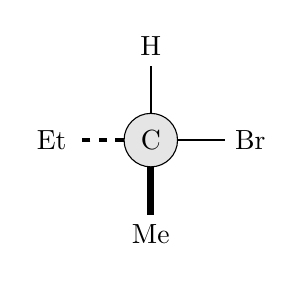
\begin{tikzpicture}[scale=0.8]
          \node[circle, draw, fill=gray!20] (C) at (0,0) {C};
          \node[above=0.6cm of C] (H) {H};
          \node[left=0.6cm of C] (Et) {Et};
          \node[right=0.6cm of C] (Br) {Br};
          \node[below=0.6cm of C] (Me) {Me};
          
          \draw[thick] (C) -- (Br);
          \draw[thick] (C) -- (H);
          \draw[dashed, line width=1.5pt] (C) -- (Et); % dash
          \draw[line width=2.5pt] (C) -- (Me); % wedge
        \end{tikzpicture}
        \end{center}
        The hydroxide nucleophile ($\ce{HO-}$) attacks from the backside, directly opposite the $\ce{C-Br}$ bond.
        The transition state shows both the forming $\ce{C-OH}$ bond and the breaking $\ce{C-Br}$ bond as partial bonds:
        \[
          \left[ \ce{HO} \cdots \text{C(H)(Me)(Et)} \cdots \ce{Br} \right]^{\delta-}
        \]
        The three non-reacting groups ($-\ce{H}$, $-\ce{CH3}$, $-\ce{CH2CH3}$) pass through a planar transition state geometry.
        As the bromide ion departs, the groups bend in the opposite direction.
        Since the attack is strictly backside, the configuration is completely inverted. The product is **(R)-2-butanol**:
        \begin{center}
        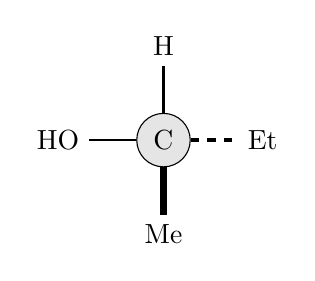
\begin{tikzpicture}[scale=0.8]
          \node[circle, draw, fill=gray!20] (C) at (0,0) {C};
          \node[above=0.6cm of C] (H) {H};
          \node[left=0.6cm of C] (OH) {HO};
          \node[right=0.6cm of C] (Et) {Et};
          \node[below=0.6cm of C] (Me) {Me};
          
          \draw[thick] (C) -- (OH);
          \draw[thick] (C) -- (H);
          \draw[line width=2.5pt] (C) -- (Me); % wedge
          \draw[dashed, line width=1.5pt] (C) -- (Et); % dash
        \end{tikzpicture}
        \end{center}
\end{enumerate}
\end{problembox}

\newpage

% ─── Section: Problems ───────────────────────────────────────────────────────
\section{Part 6 --- Problems}

\begin{problembox}
\begin{enumerate}[label=\textbf{P\arabic*.}]
  \item \textbf{Substrate and Mechanism Identification.}
  
        Predict whether each of the following substitution reactions proceeds predominantly via an $S_N1$ or $S_N2$ mechanism, and write the expected rate law:
        \begin{enumerate}[label=(\alph*)]
          \item 1-bromopropane with sodium iodide in acetone:
                \[
                  \ce{CH3CH2CH2Br + NaI -> CH3CH2CH2I + NaBr}.
                \]
          \item *tert*-butyl bromide in water:
                \[
                  \ce{(CH3)3CBr + H2O -> (CH3)3COH + HBr}.
                \]
        \end{enumerate}

  \item \textbf{Elimination Regioselectivity.}
  
        When 2-bromobutane is treated with a strong base like sodium ethoxide ($\ce{NaOCH2CH3}$), it undergoes an $E2$ elimination.
        \begin{enumerate}[label=(\alph*)]
          \item Draw the chemical structures of the two possible alkene products (1-butene and 2-butene).
          \item Identify which is the major product according to Zaitsev's rule, and explain the thermodynamic reason why this product is favored.
        \end{enumerate}
\end{enumerate}
\end{problembox}

\newpage

% ─── Section: Deep Problems ──────────────────────────────────────────────────
\section{Part 7 --- Deep Problems}

\begin{deepbox}
\begin{enumerate}[label=\textbf{D\arabic*.}]
  \item \textbf{Solvent Effects on Kinetics.}
  
        The rate of substitution reactions depends heavily on the solvent choice.
        * **Polar Protic Solvents** (e.g., water, ethanol) possess hydrogen-bonding groups. They form strong solvation shells around negative nucleophiles (like $\ce{OH-}$ or $\ce{Cl-}$), lowering their ground state energy.
        * **Polar Aprotic Solvents** (e.g., acetone, DMSO) cannot hydrogen bond, leaving nucleophiles "naked" and highly reactive.
        
        \begin{enumerate}[label=(\alph*)]
          \item Explain why polar protic solvents favor the $S_N1$ mechanism. \textit{Hint: Think about how the solvent's hydrogen-bonding ability stabilizes the leaving group ($\ce{X-}$) as it departs, lowering the activation energy for the rate-determining step.}
          \item Explain why polar aprotic solvents accelerate the rate of $S_N2$ reactions by several orders of magnitude compared to polar protic solvents.
        \end{enumerate}

  \item \textbf{Carbocation Rearrangements.}
  
        Because carbocations are unstable intermediates, they are prone to rearrange if a more stable carbocation can be formed.
        When 3-methyl-2-butanol is treated with concentrated hydrochloric acid, the major product is 2-chloro-2-methylbutane, rather than the expected 2-chloro-3-methylbutane:
        \[
          \ce{(CH3)2CH-CH(OH)-CH3 + HCl -> (CH3)2C(Cl)-CH2-CH3 + H2O}.
        \]
        \begin{enumerate}[label=(\alph*)]
          \item Draw the structure of the carbocation intermediate formed immediately after protonation and loss of water. Identify if it is primary, secondary, or tertiary.
          \item This secondary carbocation undergoes a **1,2-hydride shift** (the migration of a hydrogen atom with its pair of bonding electrons from the adjacent carbon).
                Draw the structure of the resulting carbocation after the hydride shift. Identify its class.
          \item Write the complete curved arrow mechanism for the reaction, showing the initial formation of the secondary carbocation, the hydride shift, and the final attack by the chloride ion.
        \end{enumerate}
\end{enumerate}
\end{deepbox}

\newpage

% ─── Section: Reflection ─────────────────────────────────────────────────────
\section{Part 8 --- Reflection}

\begin{reflectionbox}
\textbf{Conceptual Reflection}

Consider the following questions:
\begin{enumerate}
  \item **On Molecular Concertedness:** The $S_N2$ transition state contains two partial bonds. If the nucleophile and leaving group are both negatively charged, how does the molecule minimize the electrostatic repulsion in this transition state? (Why is the backside attack angle of exactly $180^\circ$ required?)
  \item **On the Limits of Kinetics:** We saw that tertiary substrates undergo substitution via $S_N1$ because steric hindrance makes the concerted $S_N2$ path impossible. If we could physically squeeze the nucleophile past the methyl groups, would the $S_N2$ path become faster than the $S_N1$ path?
  \item **On Synthetic Design:** Organic chemistry is the architecture of molecules. Why is understanding the exact stereochemical outcome (inversion vs. racemization) of substitution reactions essential when designing a multi-step synthesis of a drug?
\end{enumerate}
\{Note: Louis Pasteur's hand-sorted tartaric acid crystals are the historical milestone that made enantiomeric resolution and drug-receptor stereochemistry possible.\}
\end{reflectionbox}

\medskip
\noindent\textbf{Looking back at Journey 6.}
You have traversed the foundations of organic chemistry:
* **Module 6.1:** Carbon geometries, $sp^3, sp^2, sp$ hybridizations, $\sigma/\pi$ bonds, and conformations.
* **Module 6.2:** Stereochemical taxonomy, chirality, R/S designations, and optical specific rotations.
* **Module 6.3:** Resonance hybrids, delocalization, Hückel's rule ($4n+2$), and the quantum particle-on-a-ring model.
* **Module 6.4:** Electron flow grammar, curved arrows, $S_N1$/$S_N2$ kinetics, and competitive $E1$/$E2$ elimination pathways.

This completes Journey 6, providing the complete mechanical grammar of organic chemistry. You are now equipped with the physical and chemical tools to explore drug design, materials engineering, and biological synthesis in the journeys ahead.

\vspace{1.4cm}
\begin{center}
{\color{JourneyColor}\rule{0.5\linewidth}{0.8pt}}\\[6pt]
{\small\color{JourneyColor}\textit{End of Journey 6 --- Organic Chemistry: Carbon's Grammar}}\\[4pt]
{\small\color{JourneyColor}You have completed the Organic Chemistry Track. Continue to: \textbf{Chemistry Journey 7 --- Organic Chemistry: The World It Builds}}\\[6pt]
{\color{JourneyColor}\rule{0.5\linewidth}{0.8pt}}
\end{center}

\end{document}
